
\chapter{绪论}
\label{chap_int}
\section{选题背景与意义}
多相流的研究在许多现代科学技术的发展上都起到了一定的指导作用,
其在水利工程、国防安全、航空航天、现代医学、核能工程等各个重要领域都有着举足轻重的地位.
科技的发展和时代的进步同样也推动着多相流的研究不断进步,使得其日益精细化与复杂化.
其中多相流的数值模拟更是凭借着自由灵活、可重复实验、耗费少等优点,
已经成功替代了许多费用昂贵、难以实现的实验,
例如:油藏量的勘测,泄洪闸室的性能研究等,图\eqref{fig:example}.
多相流的数值模拟不仅能够极大地降低科研的成本,还大大缩短了一些科学项目的研究周期.

 \begin{figure}[htbp]
 	\label{fig:example}
	\centering
	\subfigure[多相流数值模拟勘测油储量]{
		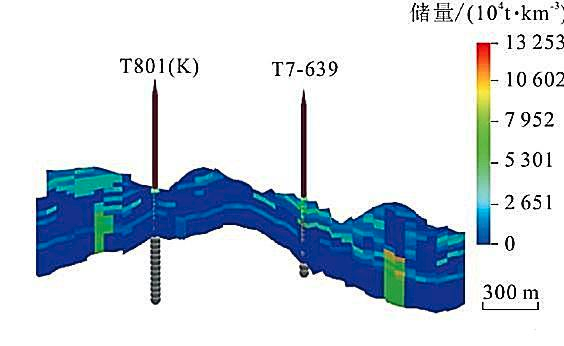
\includegraphics[width=0.45\linewidth]{images/aaa}
	}
	\hfill
	\subfigure[多相流数值模拟泄洪闸室的水流速度]{
		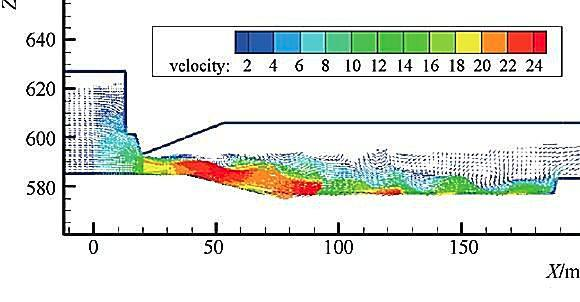
\includegraphics[width=0.45\linewidth]{images/bbb}
	}
\caption[多相流数值模拟的例子]{多相流数值模拟的例子}
\end{figure}

在多相流的数值模拟过程中,界面追踪的精度很大程度上影响了其保真度.
首先,流体自身的计算精度必然受界面追踪的误差所影响.
其次,流体曲率估算的误差与界面追踪的误差存在着密切的关系\cite{zhang17:_hfes}.
在多相流的问题研究中,有些流相的表面张力不可忽略,此时的曲率估计若不够准确,
界面上有可能产生伪波,界面因此失稳破碎,最终的计算结果也背离了物理规律\cite{denner14:comparative,francois06:balanced_force,lafaurie94:modeling}.
可见,界面追踪问题是多相流的研究中最基本且最重要的子问题之一.
然而,在许多多相流的研究中,流体界面会在几何上产生巨大的形变,
流相也可能有着潜在的拓扑变化,故界面追踪问题也因此面临着巨大的考验和挑战.




\section{现有界面追踪方法介绍}
在过去的几十年中,已经发展了许多的界面追踪法,
其中应用最广泛的三种方法分别是:
level set(LS)方法\cite{osher88:_front_propag_curvat_speed}、volume of fluids(VOF)方法\cite{Hirt.Nichols_1981_volume}
以及front tracking(FT)方法\cite{tryggvason01:_front_track_method_comput_multip_flow,unverdi92:front_tracking}.
在上述的这些方法基础上,近些年来还衍生出了一些变体方法、混合方法和自适应方法
\cite{ahn07:_multi,ahn09:_adapt,chenadec13,li03:_fixed_part_i,
diwakar09:_quadr_splin_based_inter_quasi,dyadechko05:_momen,
dyadechko08:_recon,enright02:_hybrid_partic_level_set_method,ginzburg01:_two_vof,
harvie00:_new_volum_fluid_advec_algor,
lopez04:_volum_fluid_method_based_multid,scardovelli03,
sussman99,sussman03SpectralLevelSet,sussman00:_coupl_level_set_volum_fluid,
wang12HLSVC,zhang13:VOFadvection,zhang08:_new_inter_track_method}.

\subsection{Level Set (LS)方法}
LS方法又称等值面函数法,是多相流界面追踪数值模拟的一种比较流行的方法且在许多方面都得到了应用.
LS方法最初是在1988年由美国计算数学家Stanley Osher等人提出.
LS方法的核心思想是在流场中设定一个等值面函数$\varphi(x,t)$且满足:
\begin{equation}\label{eq:LS}
\varphi_t+\mathbf{u}\cdot\bigtriangledown \varphi=0,
\end{equation}
等值面函数$\varphi$在流相交界面上的值是$0$.
在任意时刻,求解控制方程\eqref{eq:LS},得出其零等值面,便可定位流相的交界面.
LS方法不需要显式地表示界面,这一特点提高了其追踪复杂的界面的能力,
能够更容易地处理发生拓扑结构变化的情形.
由于在新的时间点,式\eqref{eq:LS}的解不再是新界面的等值面函数,
因此需要对LS函数重新初始化.
在经过有限的时间步长之后,其梯度可能变得平缓或剧烈,等值线也会因此出现聚合或者拉伸的情形,
这将使其不再继续保持距离函数的特性.
为了优化LS算法,Osher等人又对LS重新初始化的方法进行了深入研究.
考虑到边界只在某一局部区域内改变位置,故可以仅在该较小区域上求解LS方程,
这个方法被称为快速局部LS方法.
快速局部 LS方法大大加快了界面追踪的计算效率,同时也缩小了计算的存储量,提高了其实用性.
LS方法现如今已应用于多个行业,用来解决曲面重建、图像处理、最优化等各类问题.

\subsection{Volume of Fluids (VOF) 方法}
1981年,Hirts和Nichols在论文中首次提出了VOF方法,
该论文对于溃坝和涌浪的界面追踪问题进行了数值模拟.
VOF方法自提出以来,其基本思想受到广泛重视,
尤其是为输运界面的重构提供了开创性的思路.

VOF针对被追踪的流相M定义一个变量标记函数
\begin{equation}\label{bilevel}
f(\mathbf{x},t):=
\left\{\begin{array}{l}
1  \qquad \text{若}(\mathbf{x},t)\text{处含有流相介质},\\[0.2cm]
0  \qquad \text{若}(\mathbf{x},t)\text{处无流相介质}.\\[0.1cm]
	\end{array}\right.
	\end{equation}
对每一个控制体$\mathcal{C}_{i,j}$定义容积比
\begin{equation}
f_{i,j}(t) :=\int_{\mathcal{C}_{i,j}} \frac{1}{\|\mathcal{C}_{i,j}\|}f(\mathbf{x},t).
\end{equation}
在每一个时间步中,VOF方法可以再成两小步:
重建步根据边界控制体中的容积比和速度法向,
在边界单元中确定一条切线或多项式曲线,以此来近似流相的显式边界的位置,
用此结果得到的边界作为边界条件;
对流步则根据重建步得到的边界条件以及给定的流场条件
来重新计算获得每个控制体在该时间步内所产生的容积比的变化.
其中,许多的VOF方法以标量守恒来作为其理论依据,
\begin{equation*}
\frac{\partial f}{\partial t}+\nabla \cdot (f\mathbf{u})=0.
\end{equation*}
VOF保持了体积守恒,方便计算复杂的界面变化过程,
如波浪的翻卷、破碎、溶并等,已用于许多实际的模拟计算中.

\subsection{Front Tracking (FT)方法}
与VOF方法和LS方法相比,
FT方法则是通过完全显式的形式将界面用一个单独的非结构化的网格表示.
在二维情况中,FT方法将示踪点用直线相连接来近似边界;
在三维情况中,FT方法用三角平面组成的曲面来近似边界.
网格通过流场输送时,FT方法追踪每一个时间步示踪点的位置,
在进行追踪的过程中,网格界面在流场的作用下会产生位移并且不断地变形,
因此追踪过程中需要对网格进行不断地重构.
FT方法在追踪流相界面时,
其用于表示界面的示踪点的相邻两点之间的距离$h_L$能够远远小于流体内部尺度$h$,
这一特性让FT方法能够精确的锁定流相发生拓扑变化的时间点和位置\cite{brochu09},
使得它拥有了隐式方法所不具备的突出优势.

\section{现有界面追踪方法的局限性分析}
现有的界面追踪方法在许多方面都取得了重要的成就,
但依然存在着一些局限性.
这些局限性使得现有方法难有进展,更限制了多相流研究的发展.

第一,现有方法的计算精度往往不够高.

首先,在流场涡量强、界面变形大的多相流数值模拟中,
LS方法和FT方法界面追踪的误差大且难以保持体积守恒.
其次,当运动界面存在尖点(在边界上$C^1$不连续的点)时,
LS方法和VOF方法将难以保持其形状特征,它们会使得尖点附近趋于平滑.
即使在网格很密的情况下,这一局限性也无法得到有效的改善.
当多相流中包含三个或三个以上流相时,这样的尖点必然存在,
这意味着LS方法和VOF方法的精度会随着尖点的出现而进一步下降.
由文献\cite{zhang13:VOFadvection,zhang14:iPAM}得知,现有VOF方法以及FT方法最高只有二阶精度,
又由于尖点引起的精度下降等原因,很多二阶精度的方法实际上都没有达到二阶精度.
最后,在曲率估算方面,现有的研究\cite{cummins05,denner14:comparative}结果表明,
VOF+HF方法\cite{helmsen97,sussman03}是最精确的方法之一,
而此方法的曲率估计误差存在下界,下界会随着方法收敛阶的增加而减小.
其中对于二阶方法来说,曲率估计误差$\epsilon_{\kappa}$和
界面追踪误差$\epsilon_p$之间满足$\epsilon_{\kappa} \sim O(\sqrt{\epsilon_p})$的关系\cite{zhang17:_hfes}.
这就是说,界面追踪的有效数字有一半会丢失在曲率估计的时候,若界面追踪的精度不够高,
那对于实现曲率的准确估计就更加困难了.

第二,现有方法对于流体的拓扑变化处理无力.

LS和VOF方法将几何拓扑问题转化成了求解数值偏微分方程问题,
无须对流相的拓扑变化进行特殊处理,
这种特性虽然从某种程度上简化了问题,
但在界面追踪中回避几何拓扑的方式从长远发展上来看是治标不治本的.
从物理的角度而言,在界面追踪的过程中,当流相发生拓扑变化时,
具体的变化细节应根据流相的物理性质来考虑,
而不是简单的“自动化”就能进行统一处理的,
LS方法和VOF方法很难将流相的物理性质高精度地反应到界面追踪的算法中\cite{zhang14:iPAM}.
此外,当流速场足够连续时,相应的流函数应是同胚的,
而LS方法和VOF方法在追踪过程中可能存在改变流相拓扑的情况,
这和流函数是同胚映射的事实相违背.
最后,现有方法在处理流相的拓扑变化时可能产生较大的误差.
例如,当VOF方法在处理尺度小于控制体边长$h$的界面合并时,
每一个产生拓扑变化的控制体将造成$O(h^{\textup{D}})$的误差(D是计算域维数).
已知边界的控制体个数是$O(1/h^{\textup{D-1}})$,时间步数是$O(1/h)$,
因此当多相流的拓扑变化过于频繁时,
时间和空间上的误差累计可能会使得VOF方法的界面追踪结果不收敛.

第三,显式的界面追踪方法缺乏系统的理论分析体系.

LS方法的理论分析体系相对较完备\cite{falcone14,giga06,sethian97},
不论是在解的唯一性\cite{chen91,evans91,giga92}、稳定性,
还是对于解的收敛性\cite{barles91,crandall96,decknlnick00,falcone98,falcone01,walkington96}上都有相关的证明.
与LS方法相比,关于显式FT方法的理论分析则在文献中很少见,
这可能是因为FT方法常常需要一些不严格的假定,
在拓扑变化的处理上一般针对特定条件及特殊应用来进行算法设计.
由此可见,FT方法不具有一般普适性.


\section{文章结构}

为了突破现有方法的局限性,
MARS理论\cite{zhang13:_donat_region,zhang15:_gener_donat_region,zhang19:_boolean_algebra}
以及高阶数值方法\cite{zhang17:_hfes,zhang18:cubicMARS}应时而生,
其具备了以下特征:
\begin{enumerate}
	\setlength{\itemsep}{0pt}
	\setlength{\parsep}{0pt}
	\setlength{\parskip}{0pt}
	
	\item 在精度上,基于MARS理论和高阶数值方法的二维界面追踪法cubic MARS\cite{zhang18:cubicMARS}
	具有时空一致的四阶精度,
	且最大限度地保持了流相的几何拓扑特性, 即使在流体边界存在尖点的情况下,也能达到四阶精度\cite{zhang18:cubicMARS}.
	
	\item 在拓扑处理上,若流场足够连续,即使在流体形变很大时,
	二维界面追踪法iPAM以及cubic MARS均能在整个过程中
	保持流相的拓扑结构不变化\cite{zhang18:cubicMARS}.
	
	\item 在理论上,MARS理论框架的分析思路将显式界面追踪方法进行了统一,
	适用包括但不仅限于FT方法,MOF方法\cite{ahn09:_adapt,dyadechko05:_momen,dyadechko08:_recon},iPAM方法\cite{zhang14:iPAM}等,
	特别地对于VOF方法进行了其精度的分析证明\cite{zhang16:_mars}.
\end{enumerate}


本文将基于MARS理论的界面追踪法从二维推广到三维情况.
作为一项开创性的工作,
我们将本文的工作限制在流映射是同胚的简单情况下,
因此没有涉及拓扑变化的情况.


论文的主要结构如下:


第一章是绪论部分,具体交代了选题的背景与意义,
介绍了现有的应用广泛的几种界面追踪方法,并通过比较与分析得出了现有方法所存在的一些局限性,
介绍了MARS方法的优势及本文的主要工作.


第二章主要介绍了本文所应用的数学知识和背景,
包括三维情况中的连续介质模型,
三维界面追踪中用于表示流相界面的单纯复形以及MARS理论的基本定理定义.


第三章提出了一个三维界面追踪的linear MARS方法,
并通过误差分析证明了其二阶精度.


第四章展示了三维linear MARS方法在几个经典数值测试中的结果并展示了其二阶精度.


第五章对全文进行了总结和回顾,并提出了展望.